\newpage
\thispagestyle{empty}

\color{white}
\section*{Focus on Modeling: Spring-Mass Systems}
\normalcolor
\vspace{-24pt}
{\begin{center}
\psframebox[style=fombox]{\begin{minipage}{6in}
\begin{center}
FOCUS ON MODELING

{\huge Spring-Mass Systems}
\end{center}
\hspace{0.125in}
\index{spring-mass system}%
Second-order ODE arise when we model the behavior of a mass attached to a freely-moving end of an ideal spring, possibly subject to a damping effect (imagine the spring and mass are submerged in molasses).  Understanding this model is a first step toward being able to analyze more complicated systems of physical oscillators.

\hspace{0.125in}
Let us begin with a figure illustrating our physical system:

\begin{center}
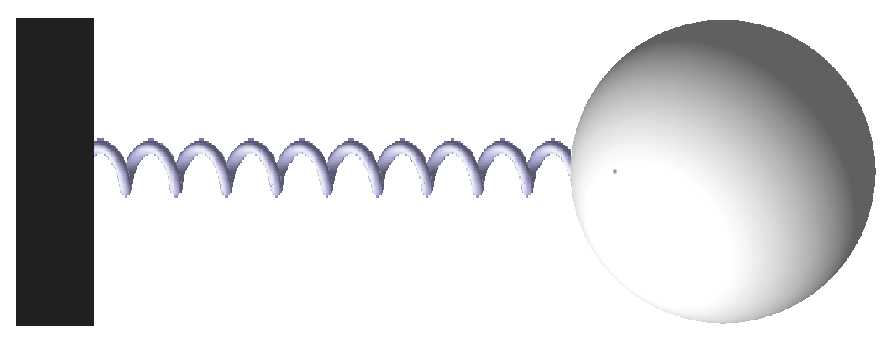
\includegraphics[width=2.5in]{FOM-springmass/springmass2smallest.eps}
\end{center}

The free end of the spring is allowed to move, and we need to impose coordinates on the figure to measure this motion.  There are many ways we could choose to do this.  The natural point to choose as an origin is the 
	\index{rest position}%
	{\bf rest position} of the free end of the spring -- that is to say, the point where the free end sits when the spring is not in a state of internal tension.  From this point, we can measure the displacement of the free end of the spring, and we shall adopt the convention that a stretched spring corresponds to a positive displacement, while a compressed spring corresponds to a negative displacement.

\begin{center}
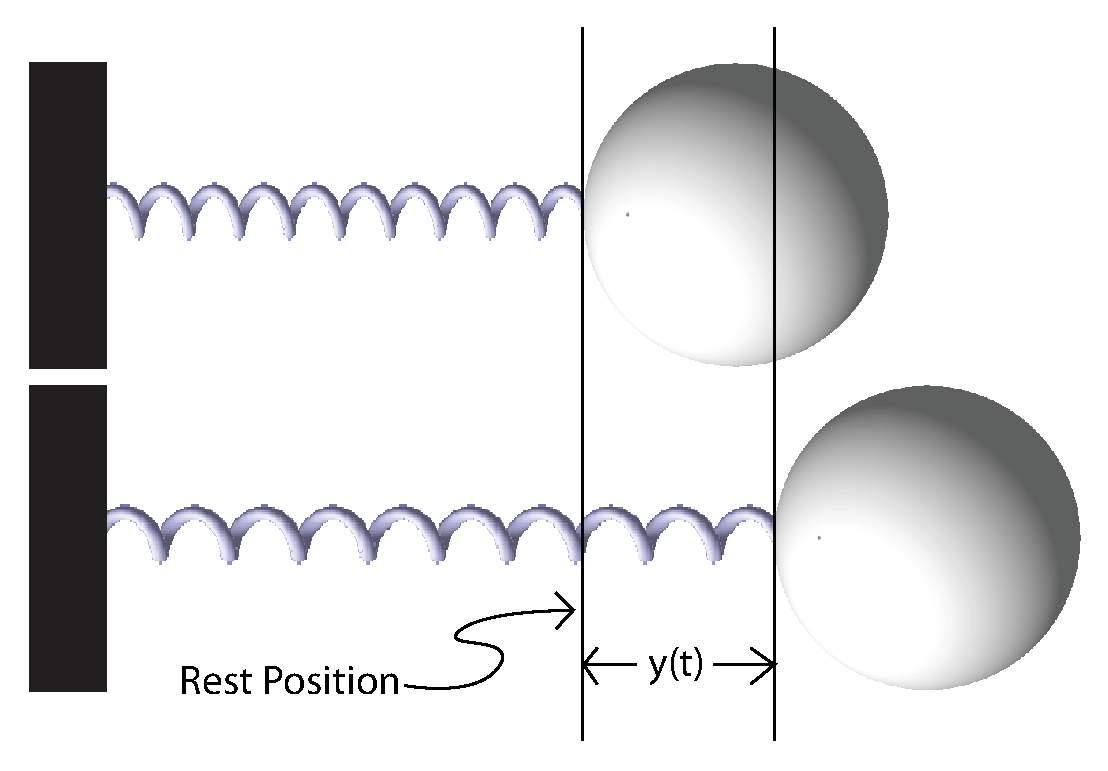
\includegraphics[width=3in]{FOM-springmass/springmassdisplacement.eps}
\end{center}

\hspace{0.125in}
To model the physical behavior of this system, our starting point is Newton's second law, $F=ma$ (force equals mass times acceleration).  If we let $y(t)$ denote the displacement of the free end of the spring from it's rest position as a function of time, then the acceleration is given by $\ddot{y}$.  There will also be at least two forces acting on the mass.  One is the spring's restoring force, which Hooke's Law tells us we can model by assuming it is proportional to the displacement from rest position: $F_s = -ky$.  (Here, the spring constant $k$ is positive, and the direction of the spring's restoring force is in the direction opposite the displacement.  Also, we will model the damping force by assuming it is proportional to the velocity of the mass (like viscous drag) and in the opposite direction: $F_d = -C\dot{y}$.  Let us denote any other external driving force by $F_e$, and suppose this driving force is described by a function of time, $F_e=f(t)$.  

\end{minipage}
}
\end{center}




\newpage
\thispagestyle{empty}

{\begin{center}
\psframebox[style=fombox]{\begin{minipage}{6in}



\hspace{0.125in}
With these conventions we have:
\[ ma=F_s+F_d+F_e\]
or
\[ m \ddot{y} = -ky - C \dot{y}+f(t),\]
which we rearrange as
\[ m \ddot{y} + C \dot{y} + k y = f(t).\]
We now see that this is a second order constant coefficient linear ODE, so we can study the behavior of this system using the mathematical techniques now available to us.  

\hspace{0.125in}
A standard choice of units for force would be Newtons, and a standard choice for measuring displacement $y$ would be meters.  Thus the spring constant could have units of $\frac{N}{m}$, indicating that the magnitude of the spring's restoring force is $k$ Newtons for each meter the spring is displaced from rest position.  If these units are used, then the last term on the left side of our ODE will have units of Newtons, which is consistent with the kind of units we would see on the right side of the equation for an external driving force $F_e$.  To maintain consistency with the other terms on the left side of the equation, we should select mass $m$ to be measured in kilograms, and time should be measured in seconds; that way the units of $m\ddot{y}$ will be $\frac{kg \cdot m}{s^2}$, which are the same as Newtons.  Similarly, the units of the damping coefficient will have to be $\frac{N \cdot s}{m}$.

\hspace{0.125in}
{\bf EXAMPLE:} Consider a mass of $3 \ kg$ attached to the end of a spring with spring constant $9 \frac{N}{m}$.  If there is no damping or outside driving force, and the mass is initially stretched $0.05 \ m$ from its rest position then released, determine how long it will take before the spring first returns to its rest position.  What will the velocity be at that instant?

\hspace{0.125in}
With the parameters $m=3$, $C=0$ and $k=9$, and the driving force $f(t)=0$, we are faced with the differential equation
\[ 3 \ddot{y} + 9 y = 0\]
and the initial conditions $y(0)=0.05$ and $\dot{y}(0)=0$.  The solution of this IVP is
\[ y(t) = 0.05 \cos (3t).\]
The free end of the spring will be at the rest position when $y(t)=0$, which will occurs when $3t = \frac{\pi}{2}+n\pi$, or $t=\frac{(2n+1)\pi}{6}$.  The smallest positive solution will be $t=\frac{\pi}{6}\approx 0.524 \ s$.  At that instant, the velocity will be $\dot{y} \left( \frac{\pi}{6} \right) = -0.15 \sin \left(\frac{\pi}{2} \right) = -0.15 \frac{m}{s}$.
\qed

\end{minipage}
}
\end{center}

